\documentclass[10pt]{article}

%defines page size and margins
\usepackage{geometry}
\geometry{
    letterpaper,
    left=1in,
    right=1in,
    top=1in,
    bottom=1in,
}

%Sets spacing for entire document
\usepackage{setspace}
\singlespacing

%Package for reducing space in between list items
\usepackage{enumitem}

%urls
\usepackage{hyperref}

%multirow for tables
\usepackage{multirow}

%Math symbols
\usepackage{gensymb}
\usepackage{siunitx}

%numberless captions
\usepackage{caption}

%Image path
\usepackage{graphicx}
\graphicspath{ {/} }

%Used for adjusting images
\usepackage[export]{adjustbox}

%For floating images
\usepackage{float}

\begin{document}
\title{Laboratory Six --- Filters}
\date{December 8, 2017}
\author{Rishabh Shah\\ 4655 4192\\ \\ Partner: Matthew Remillard}
\maketitle
\newpage

\section*{Pre-Lab}
\subsection*{First Order Filters}
\subsubsection*{Low Pass Filter}
$$f_c = \frac{1}{2\pi RC} = 33.86 Hz$$
\begin{figure}[H]
	\centering
	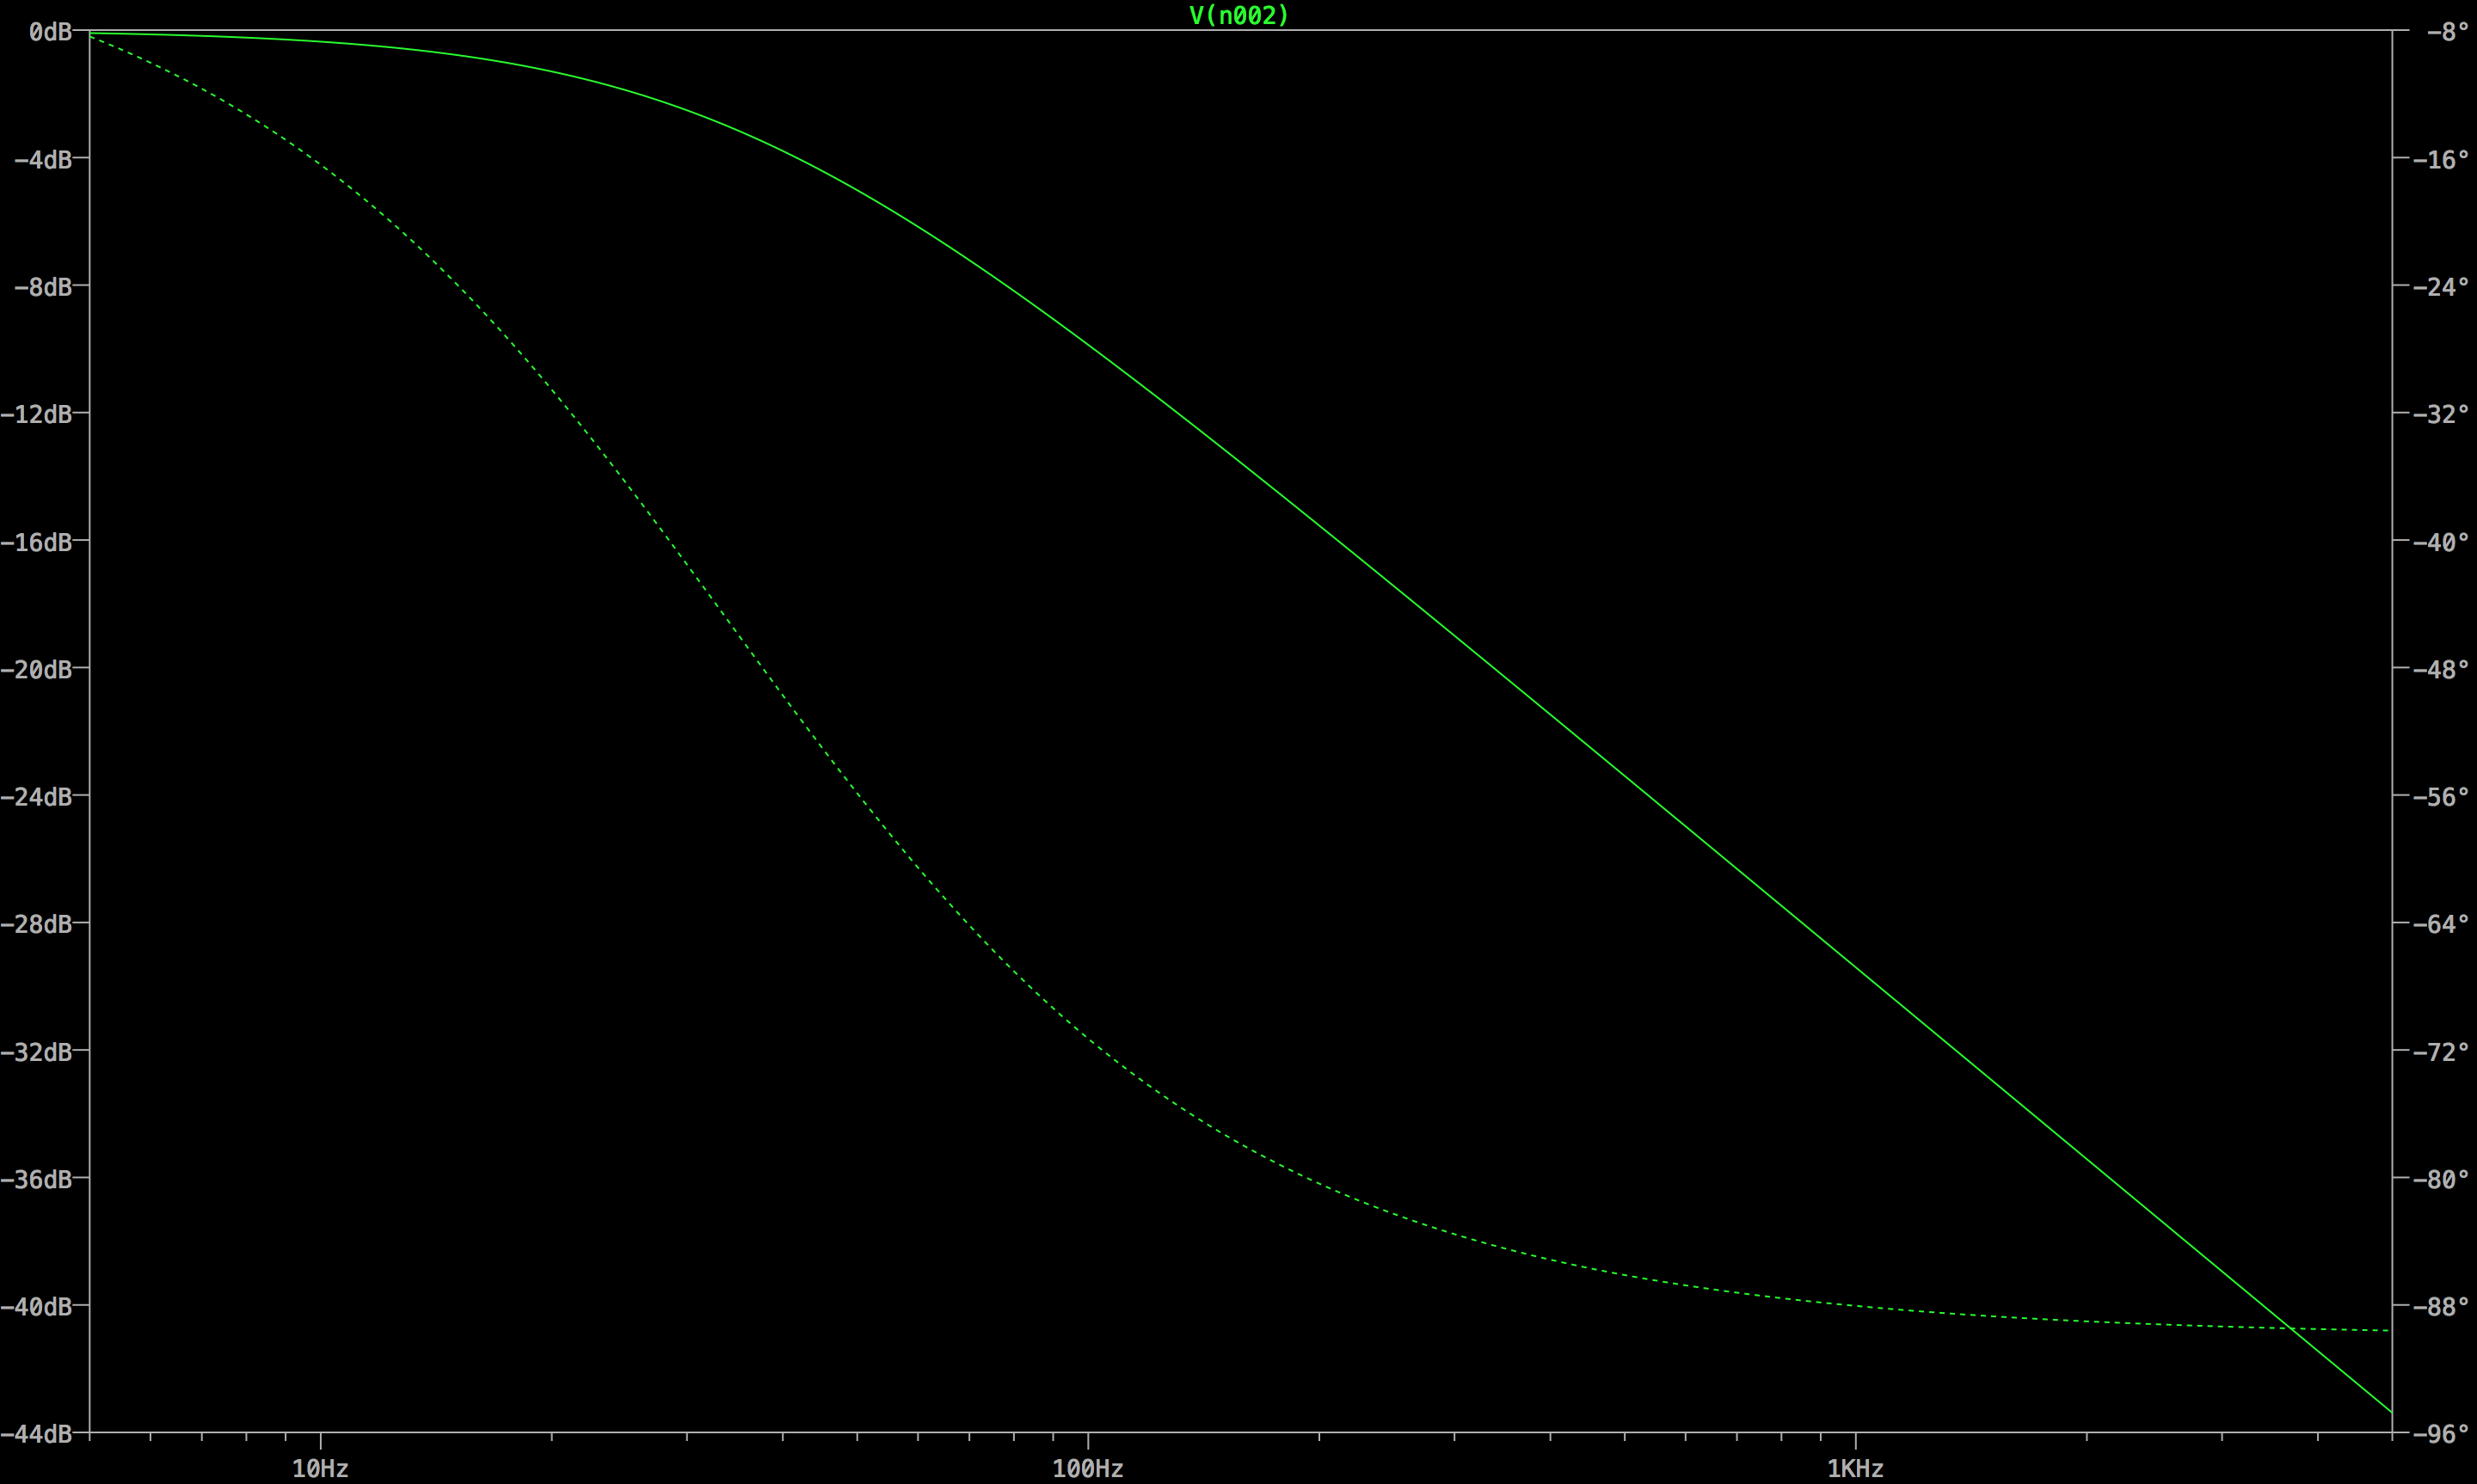
\includegraphics[width=0.5\textwidth]{PreLowPassFirst.png}
	\caption{First order low pass filter, with cutoff frequency of $\sim 33Hz$}
\end{figure}

\subsubsection*{High Pass Filter}
$$f_c = \frac{1}{2\pi RC} = 33.86 Hz$$
\begin{figure}[H]
	\centering
	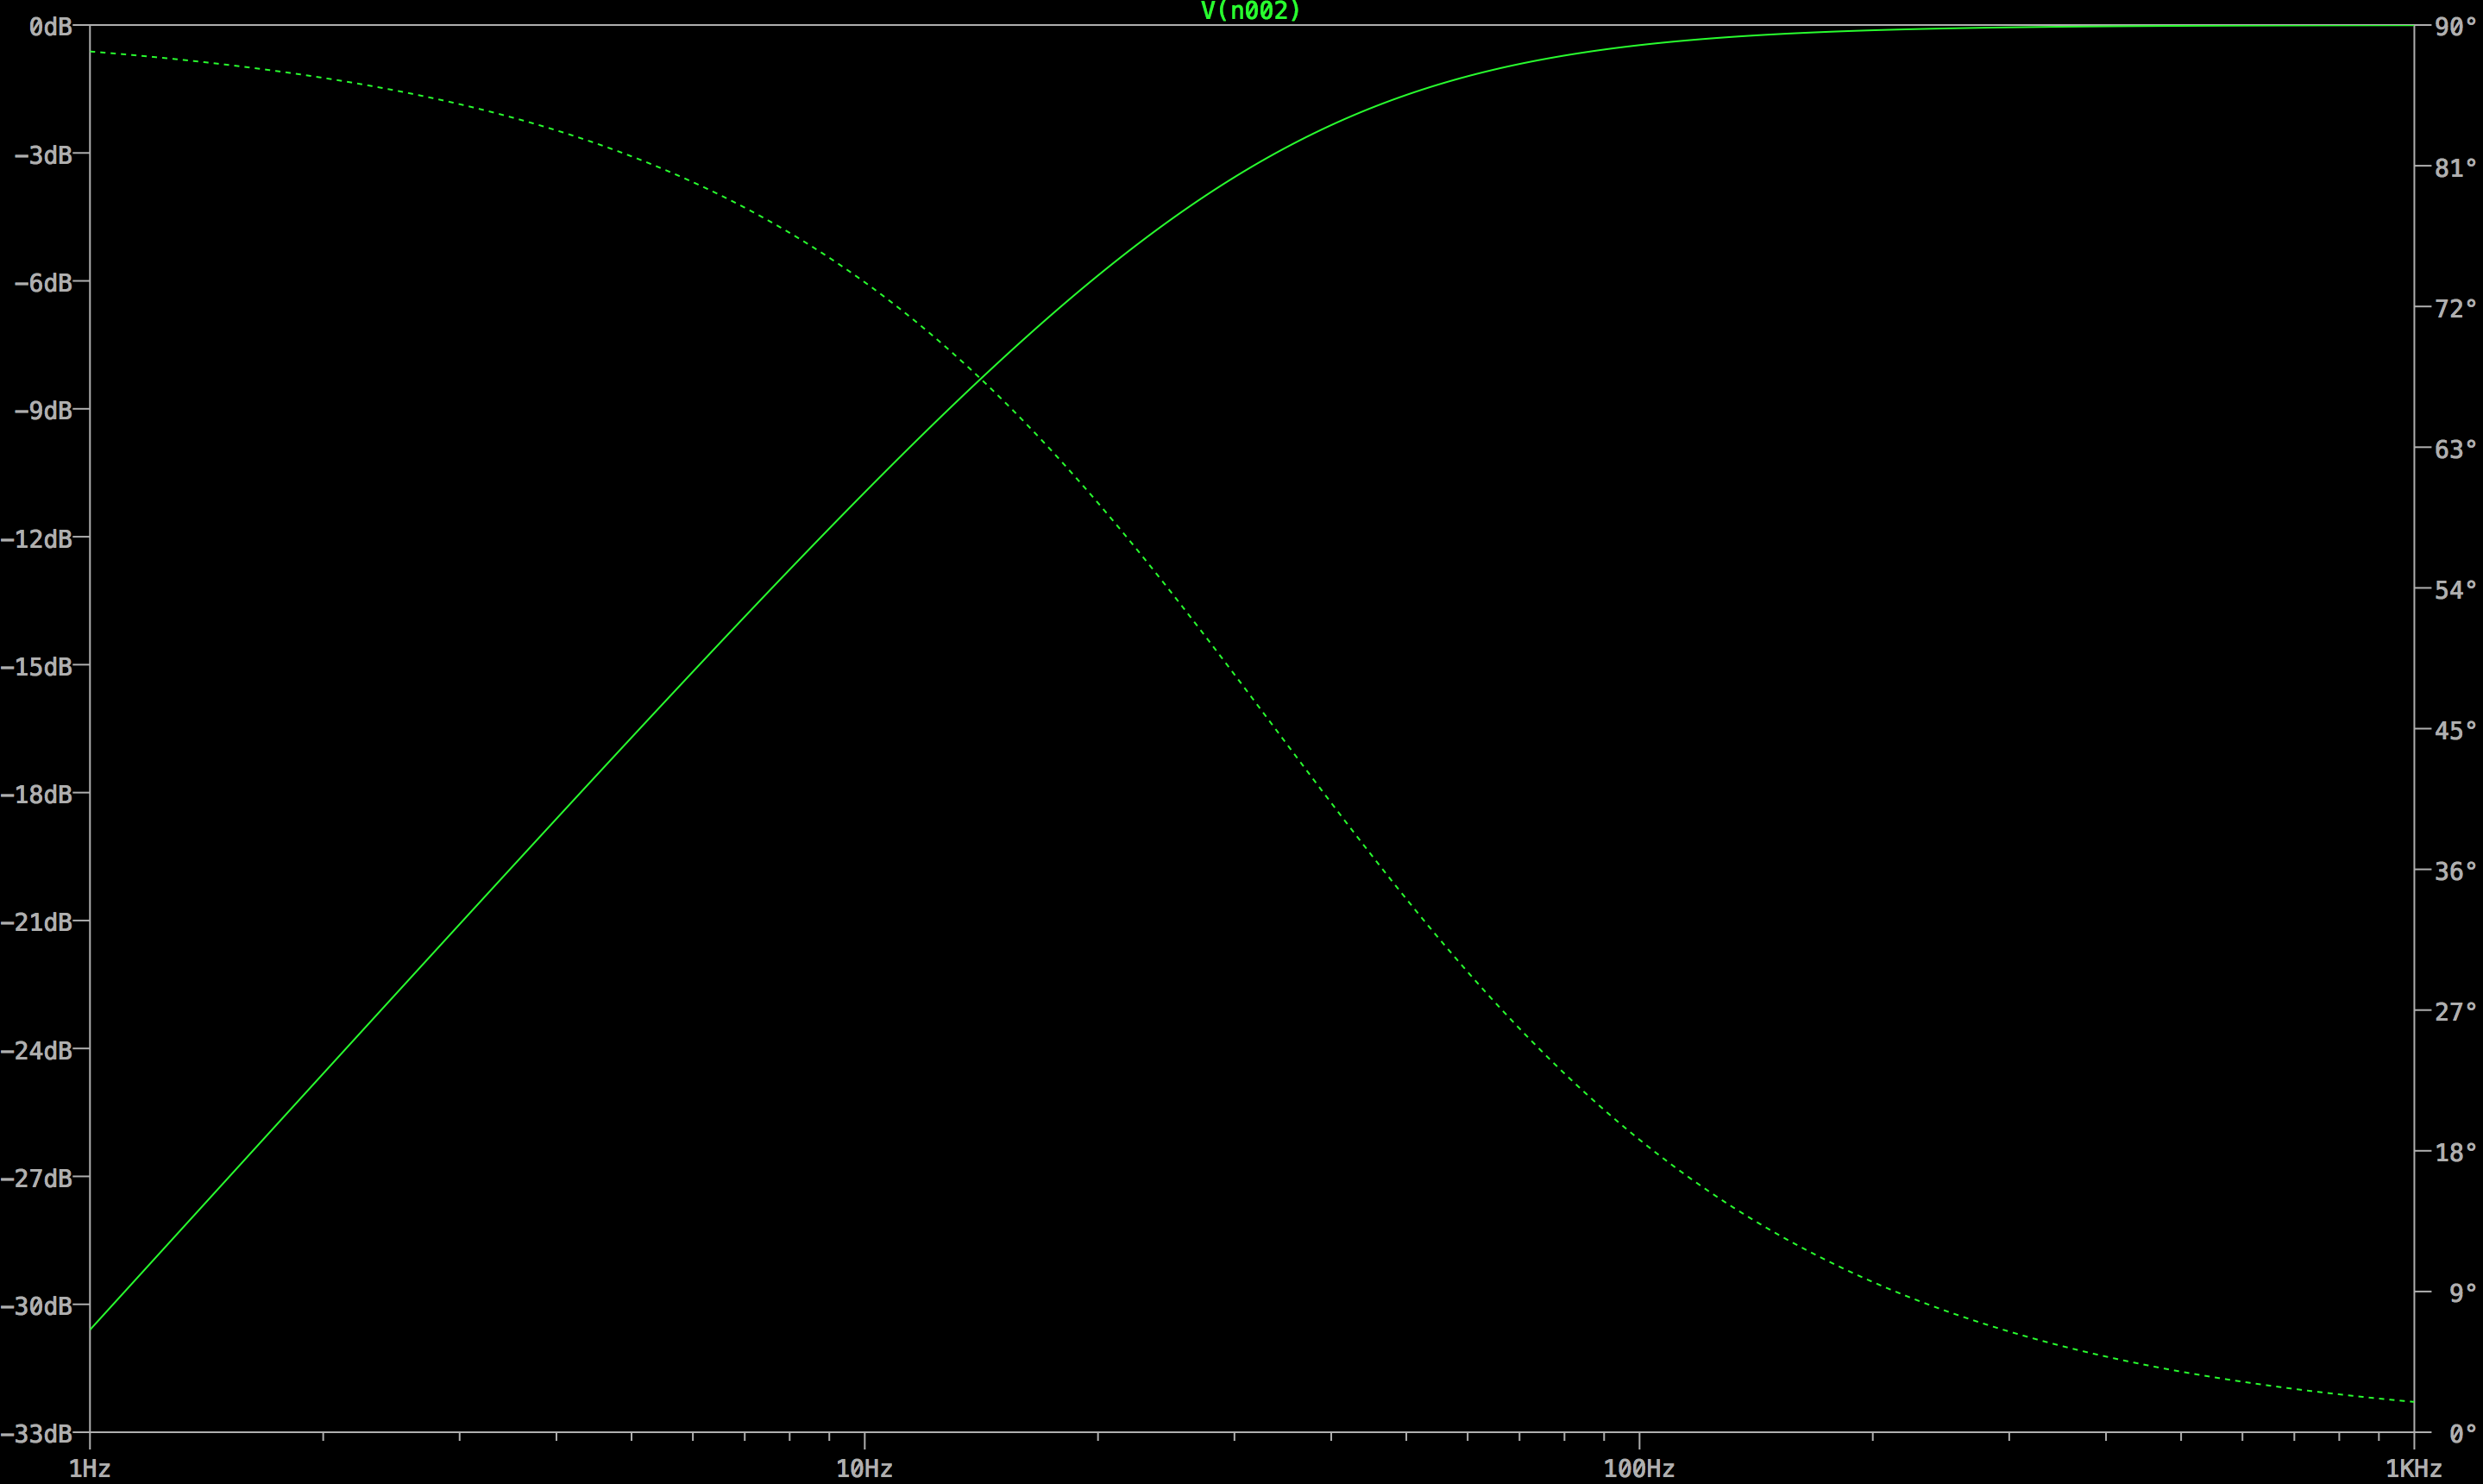
\includegraphics[width=0.5\textwidth]{PreHighPassFirst.png}
	\caption{First order high pass filter, with cutoff frequency of $\sim 33Hz$}
\end{figure}

\subsection*{Second Order Filters}
\subsubsection*{Low Pass Filter}
$$f_{MaxGainTheoretical} = 734 Hz$$
\begin{figure}[H]
	\centering
	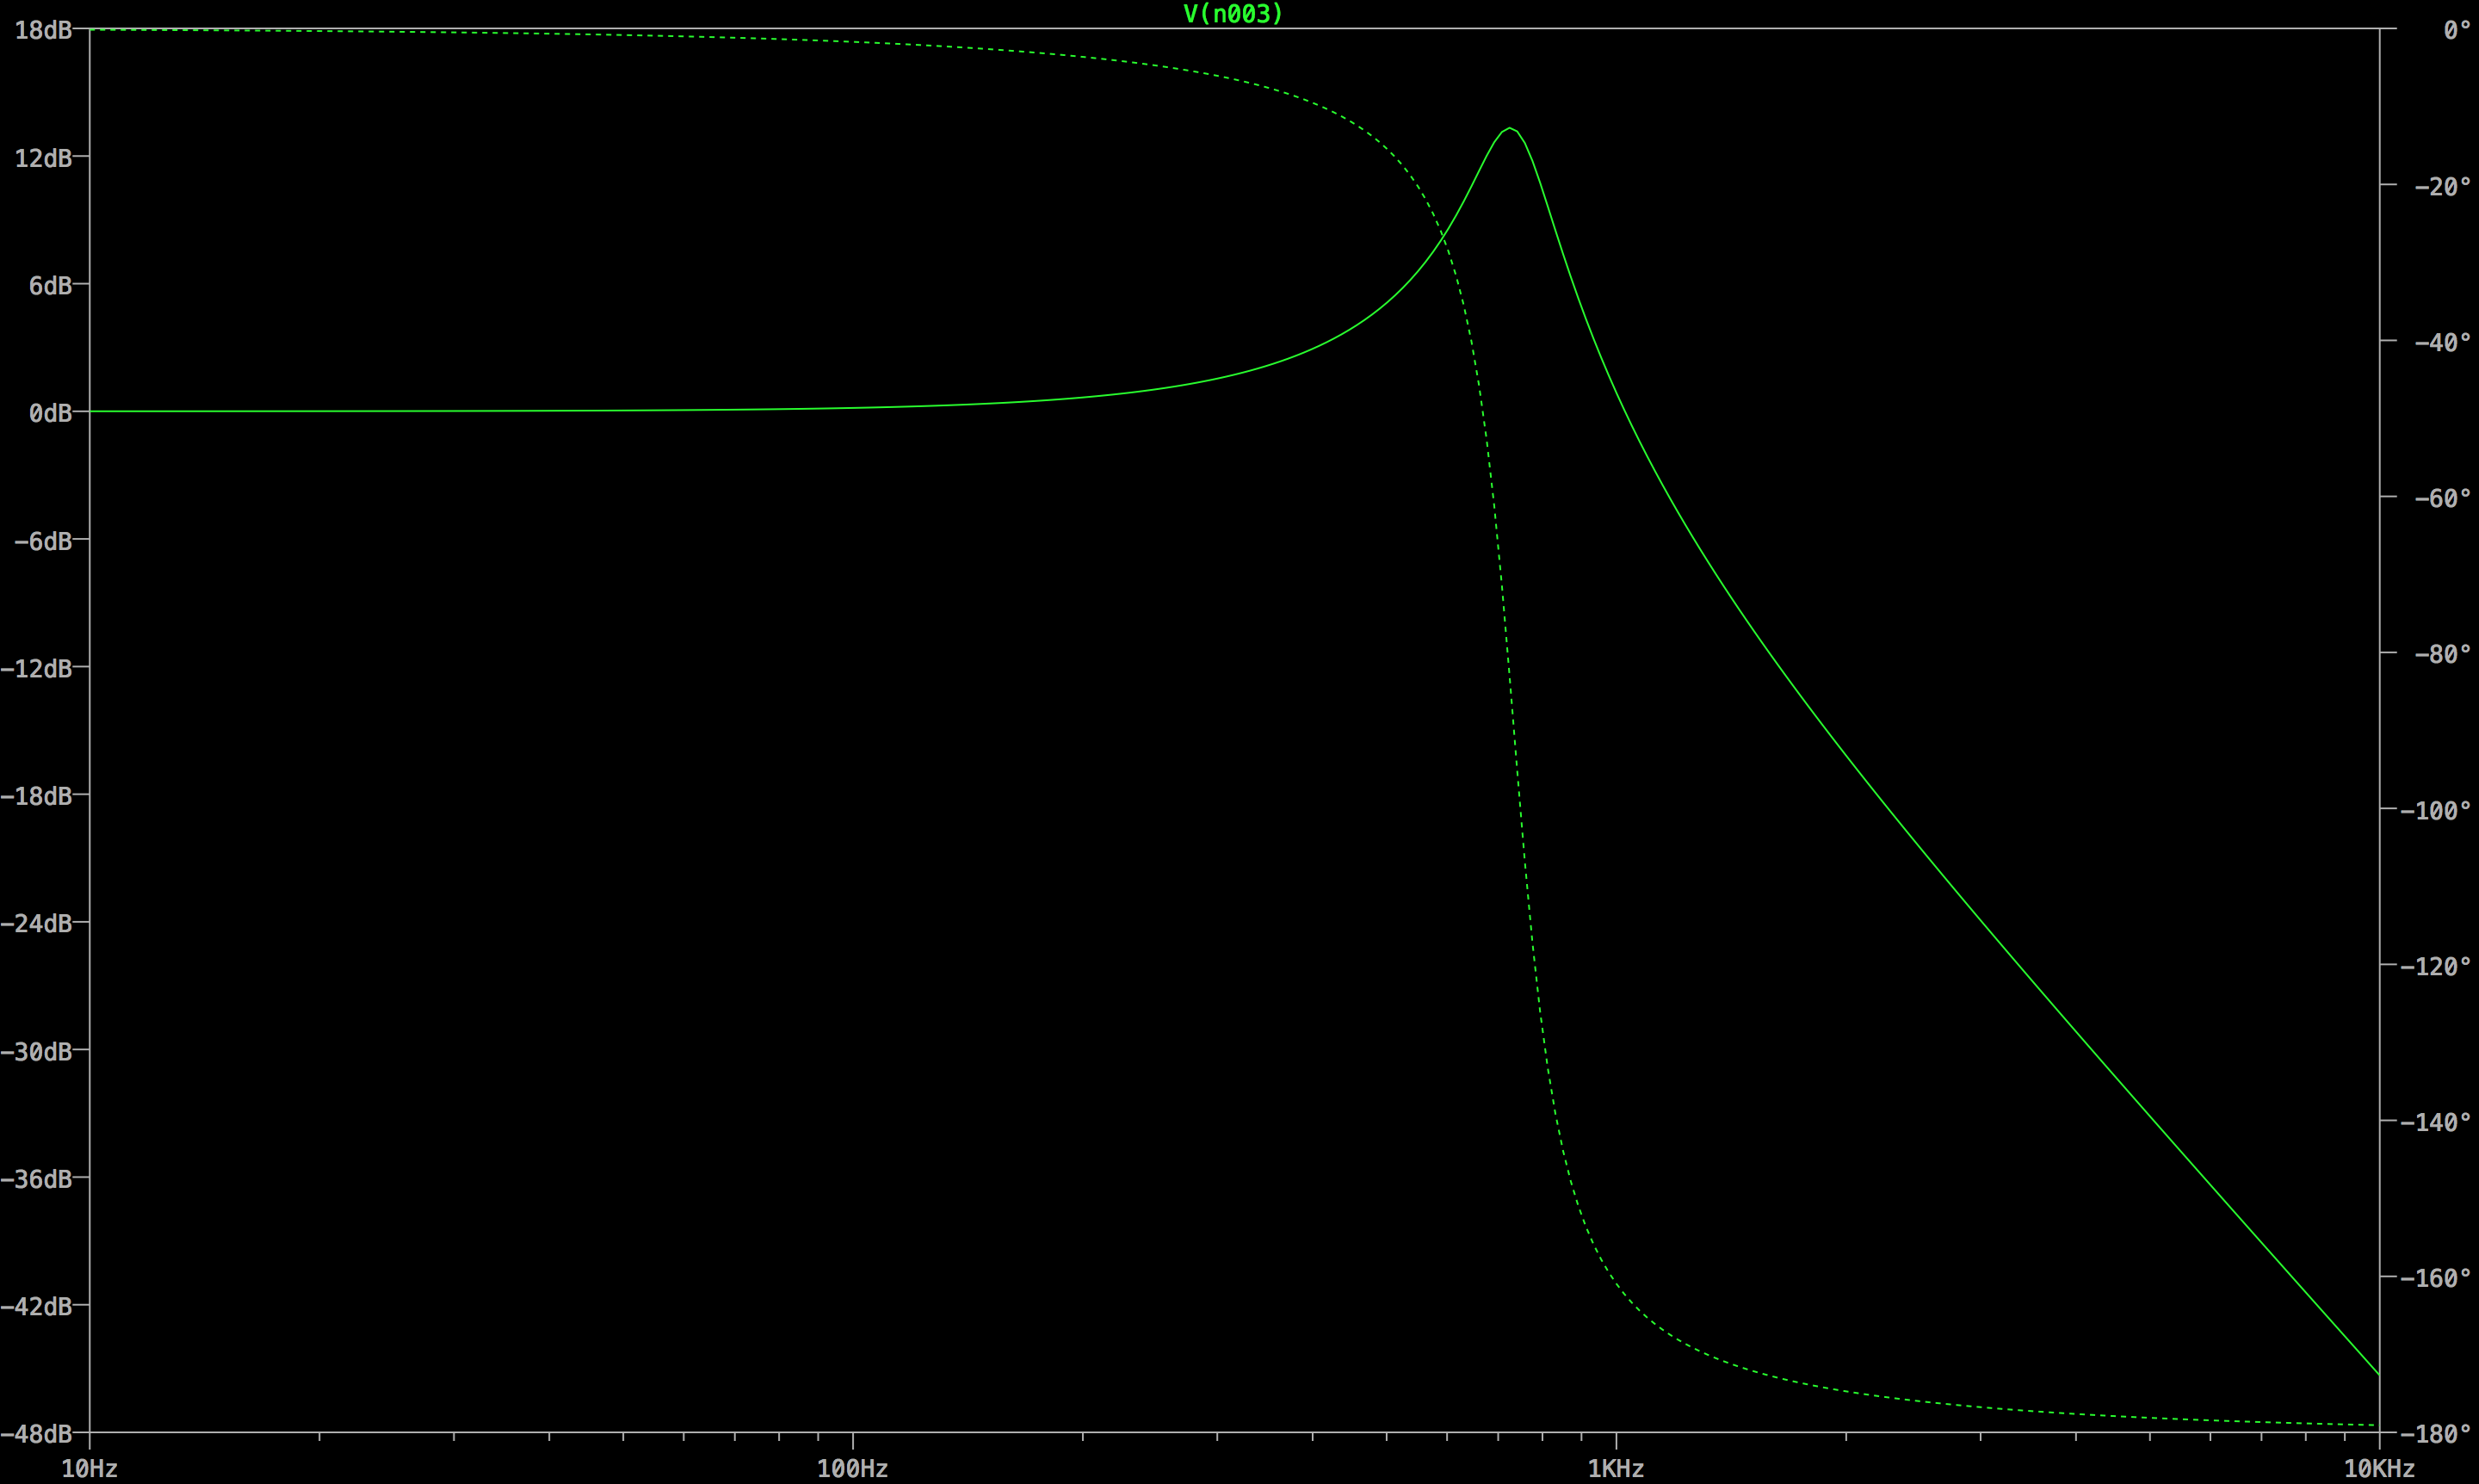
\includegraphics[width=0.5\textwidth]{PreLowPassSecond.png}
	\caption{Second order low pass filter, with maximum gain frequency of $\sim 740Hz$}
\end{figure}

\subsubsection*{High Pass Filter}
$$f_{MaxGainTheoretical} = 734 Hz$$
\begin{figure}[H]
	\centering
	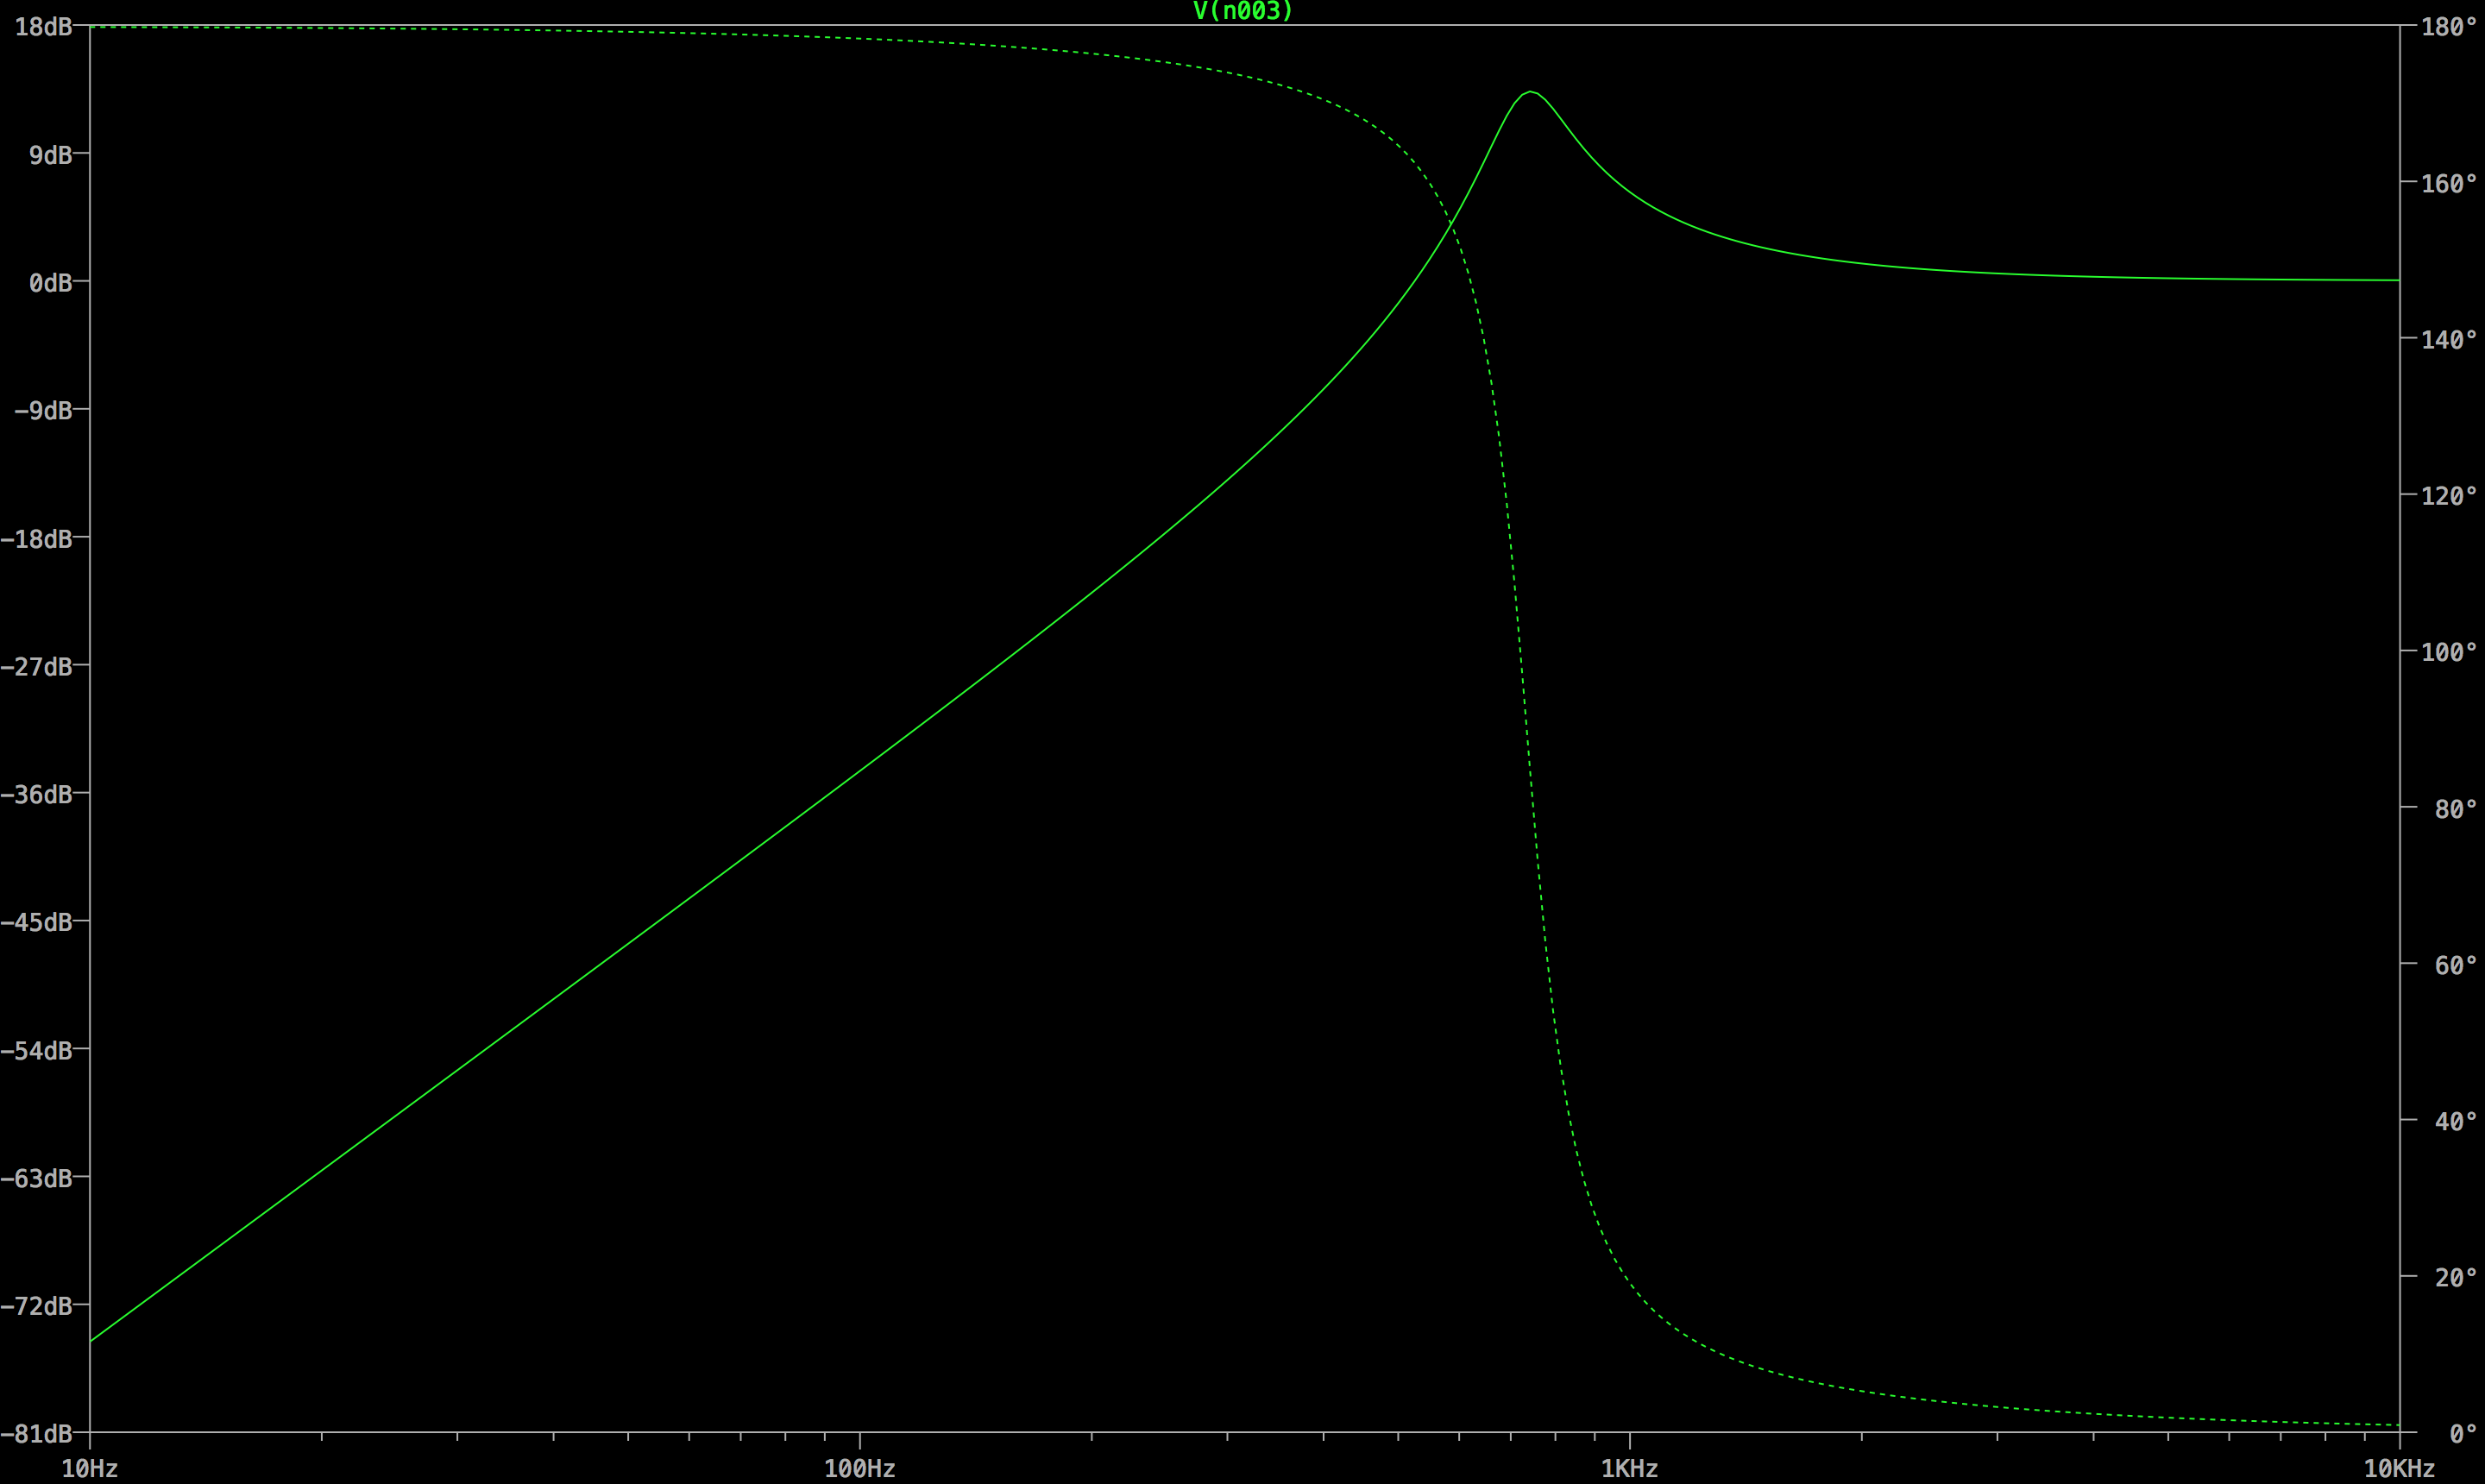
\includegraphics[width=0.5\textwidth]{PreHighPassSecond.png}
	\caption{Second order high pass filter, with maximum gain frequency of $\sim 740Hz$}
\end{figure}

\subsubsection*{Band Pass Filter}
$$f_{MaxGainTheoretical} = 734 Hz$$
$$f_{Bandwidth} = 1600Hz$$
\begin{figure}[H]
	\centering
	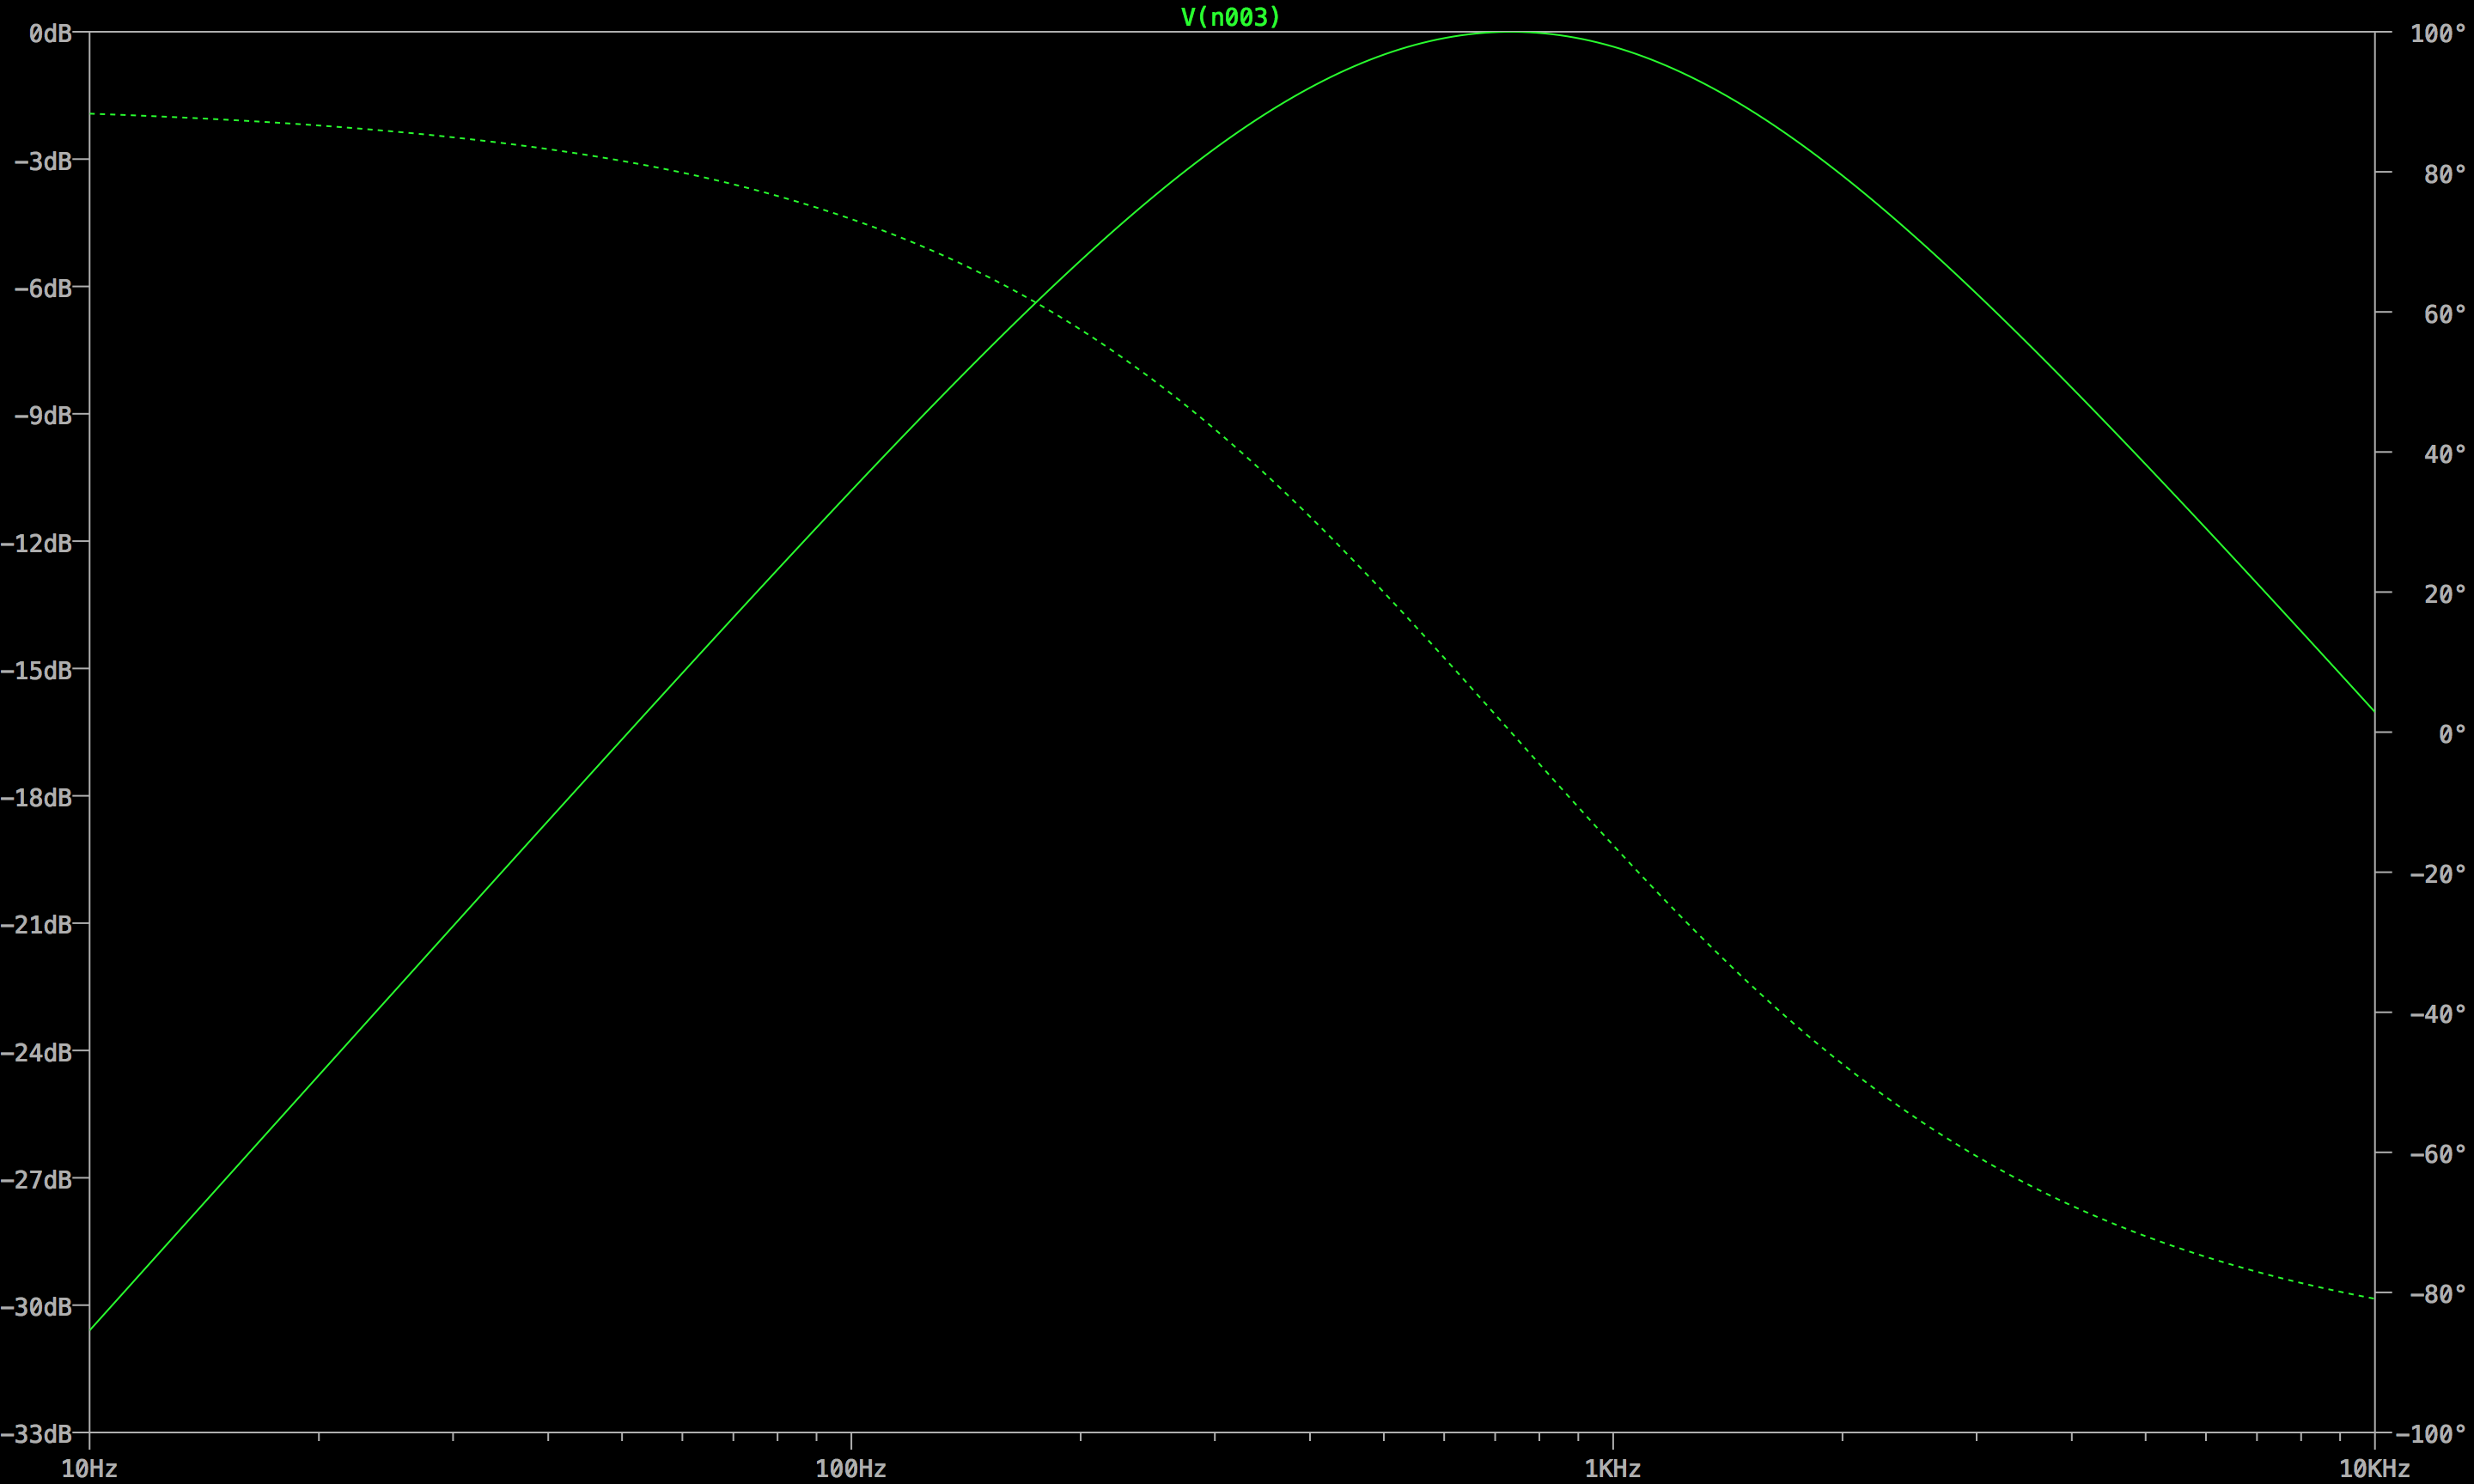
\includegraphics[width=0.5\textwidth]{PreBandPass.png}
	\caption{Second order band pass filter, with maximum gain frequency of $\sim 735Hz$}
\end{figure}

\subsubsection*{Band Reject Filter}
$$f_{MaxGainTheoretical} = 734 Hz$$
$$f_{Bandwidth} = 1591Hz$$
\begin{figure}[H]
	\centering
	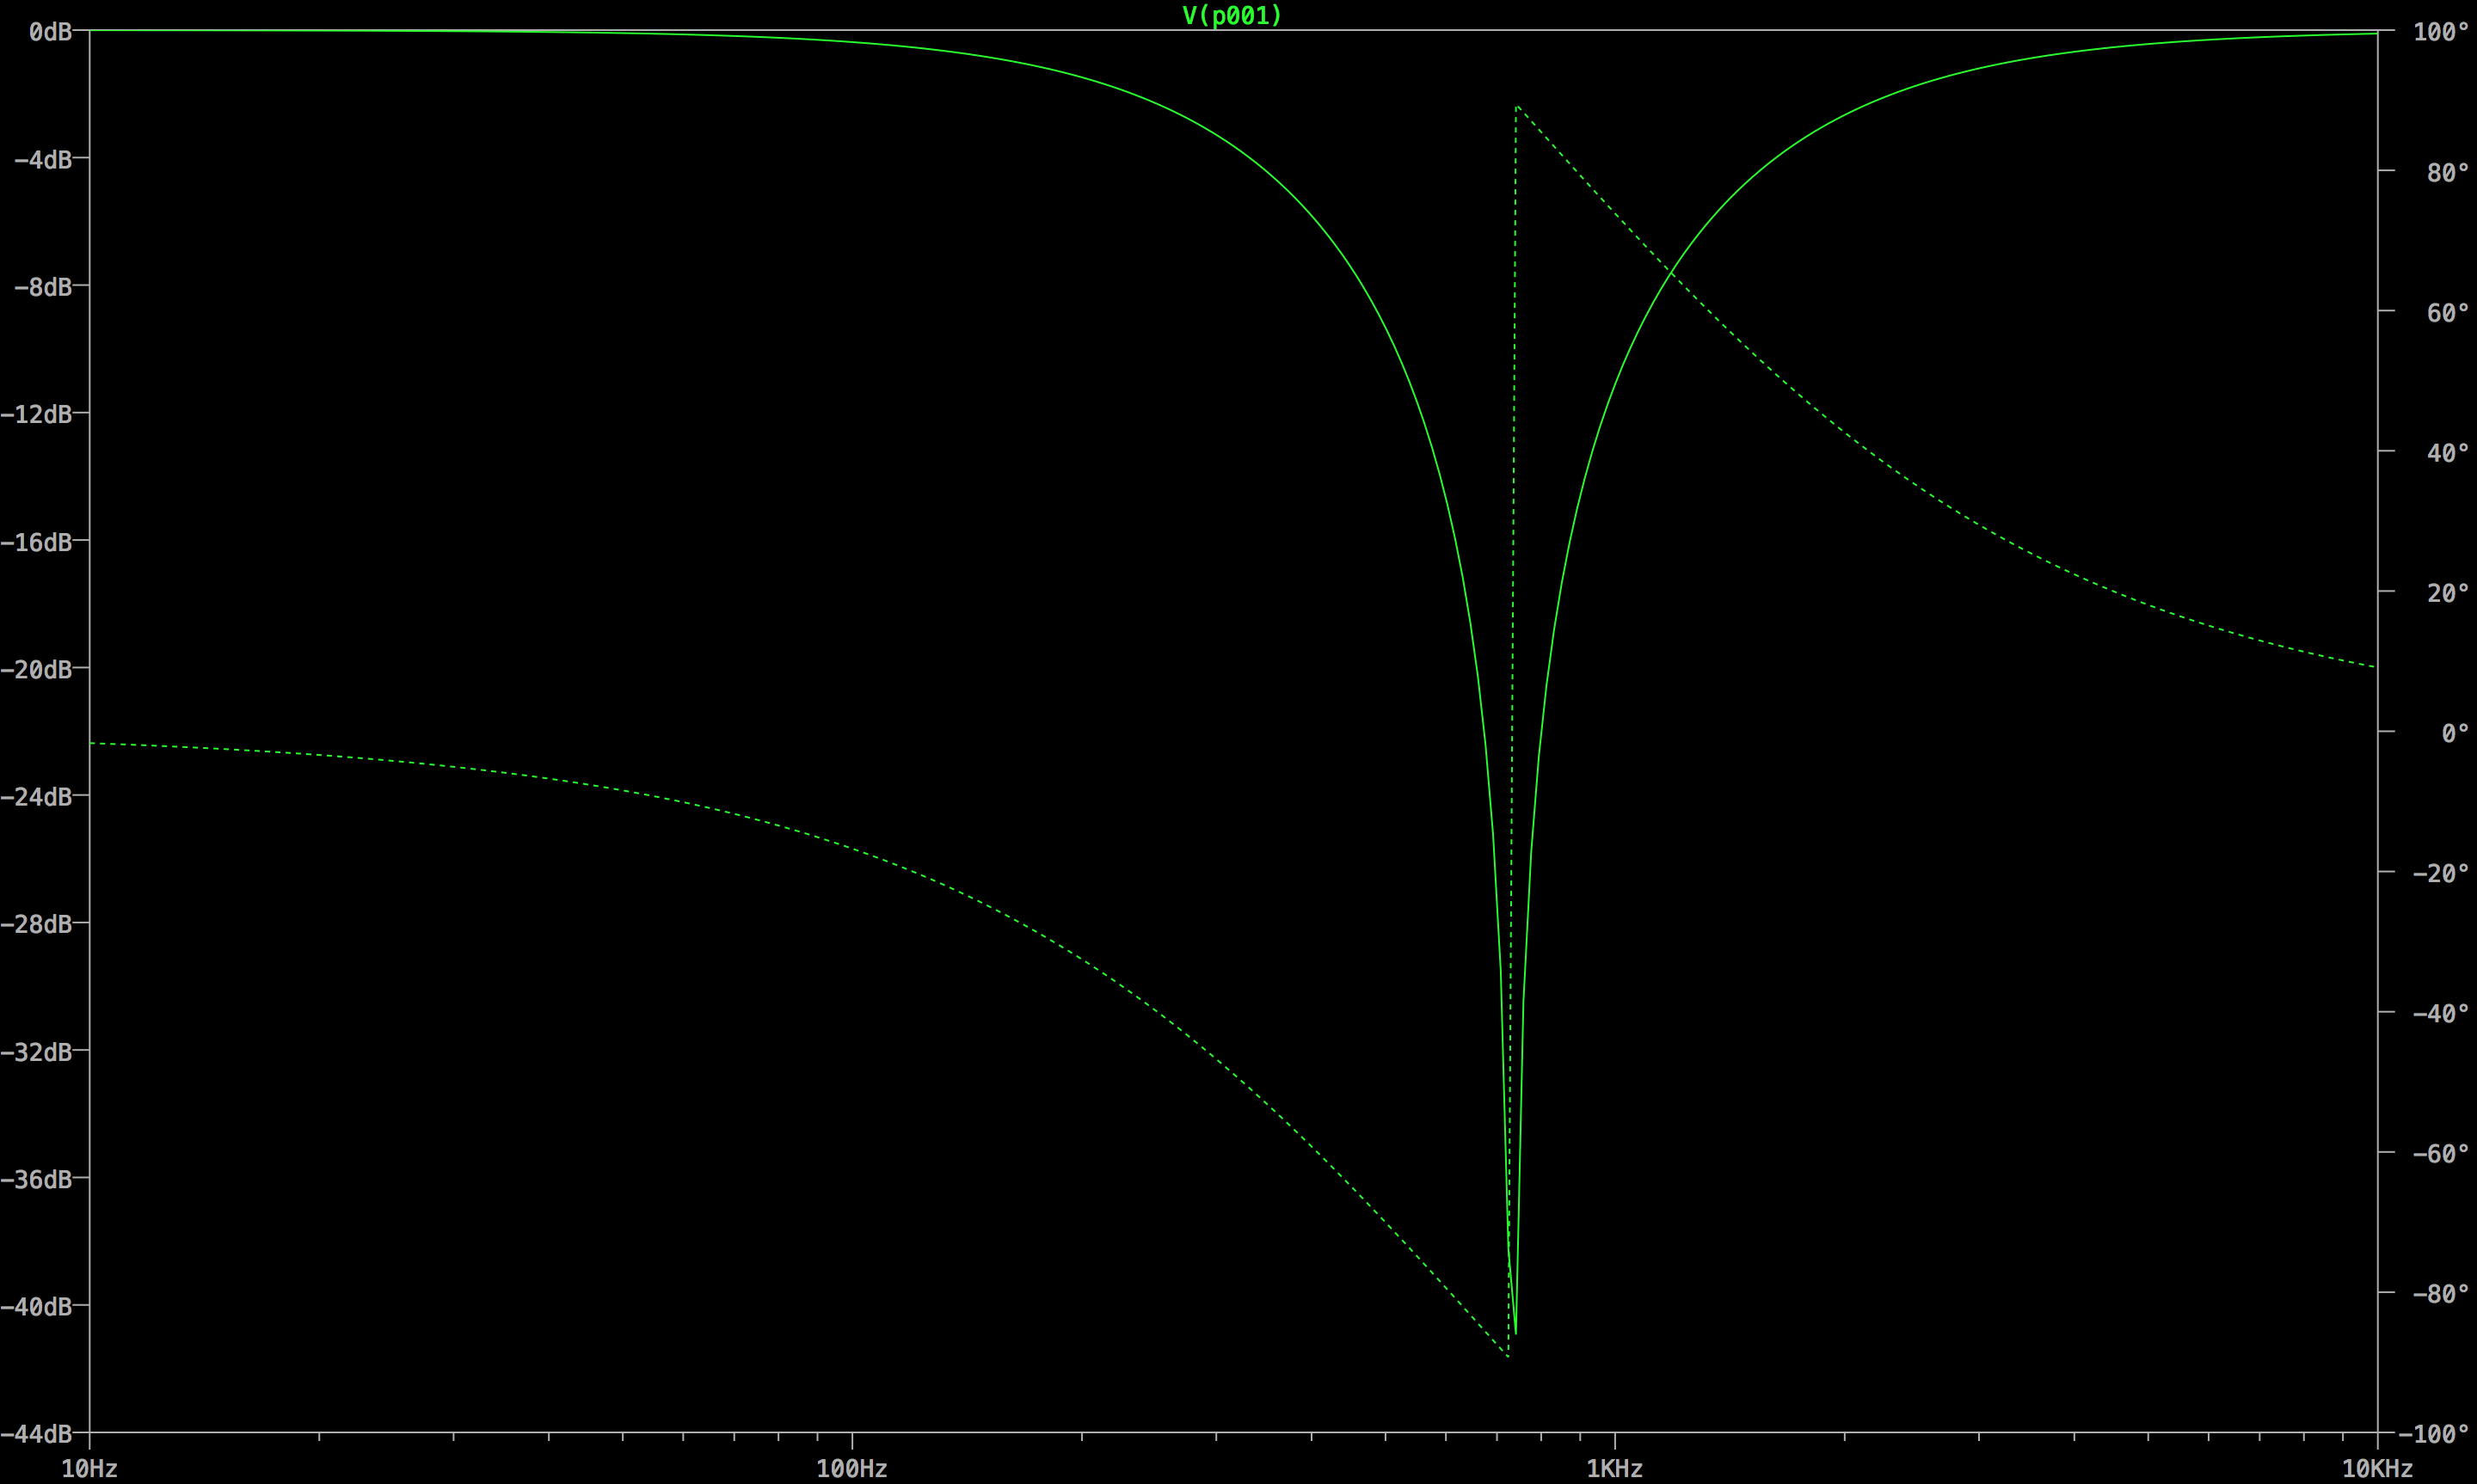
\includegraphics[width=0.5\textwidth]{PreBandReject.png}
	\caption{Second order band reject filter, with maximum gain frequency of $\sim 735Hz$, and bandwidth of $\sim 1589Hz$}
\end{figure}

\subsection*{Active Filters}
\subsubsection*{Low Pass Filter}
$$f_c = 32Hz$$
\begin{figure}[H]
	\centering
	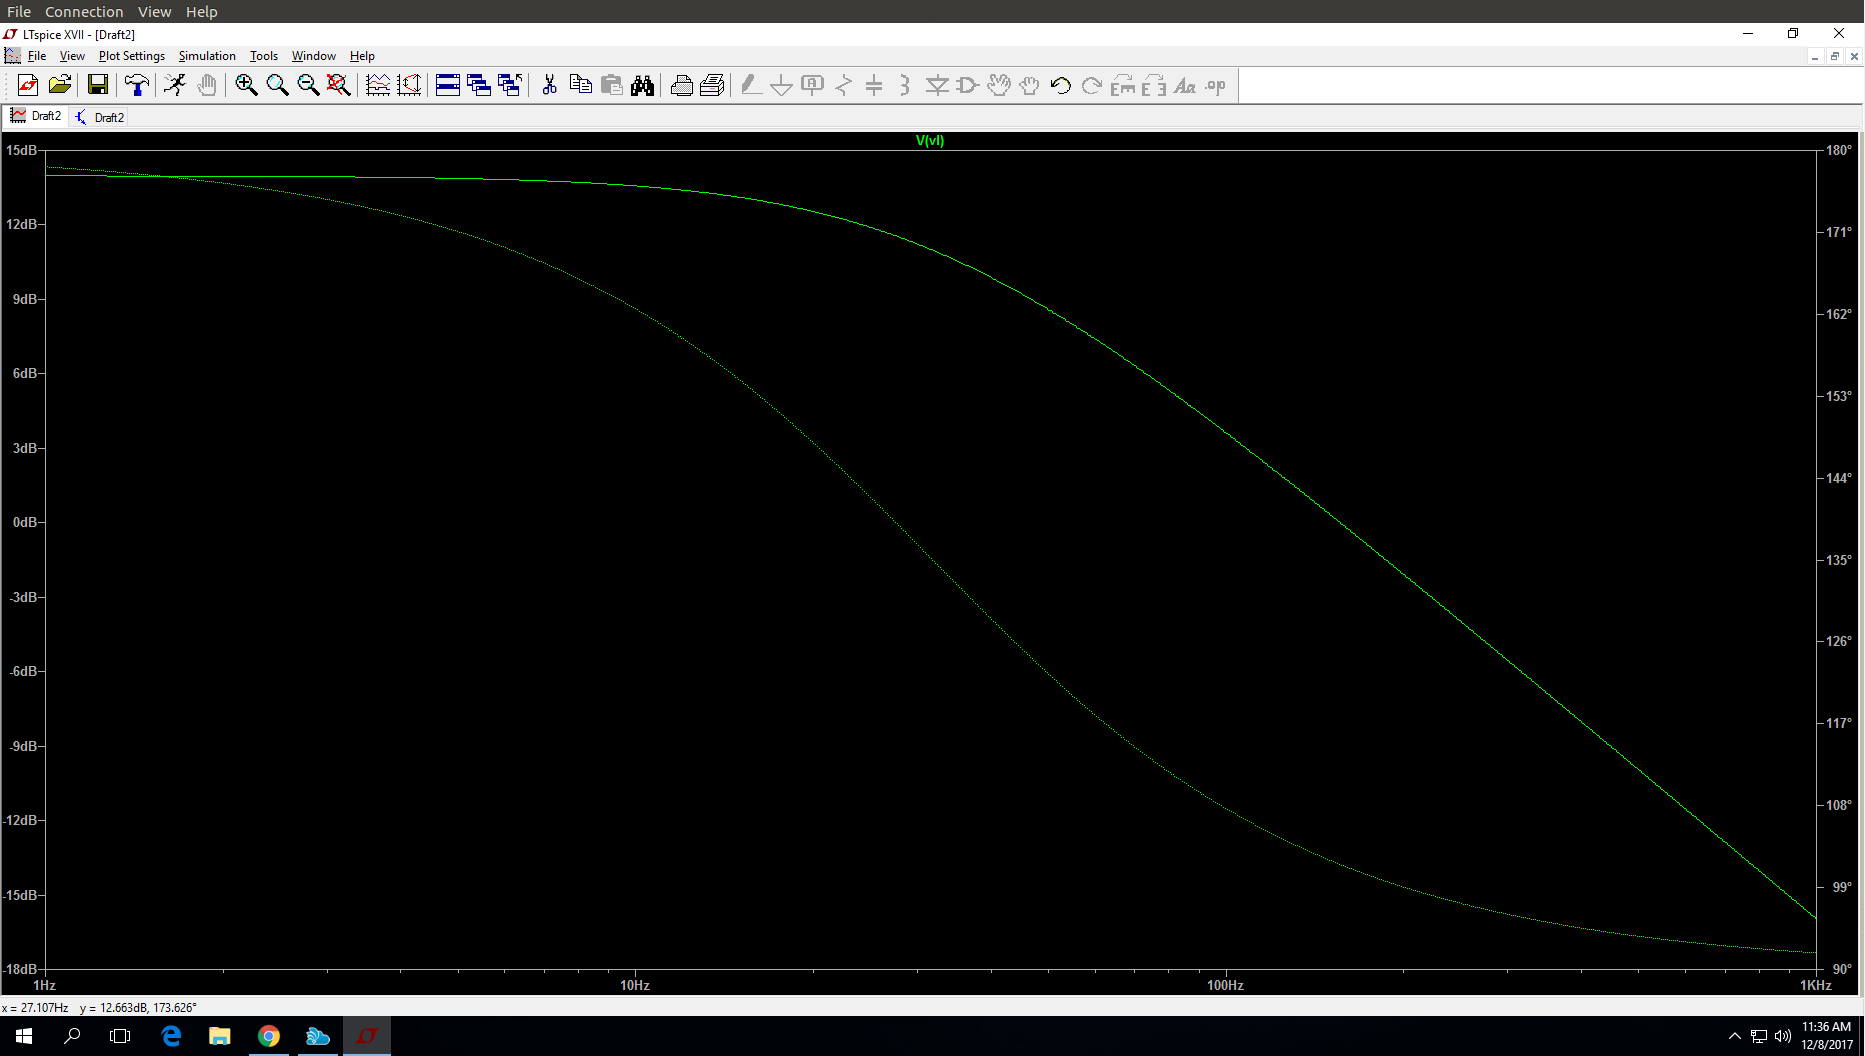
\includegraphics[width=0.5\textwidth]{PreOpAmp.png}
	\caption{Active low pass filter}
\end{figure}

\section*{Lab Data}
\subsection*{First Order Low Pass Filter}
$$f_c = 33.59Hz$$
\begin{figure}[H]
	\centering
	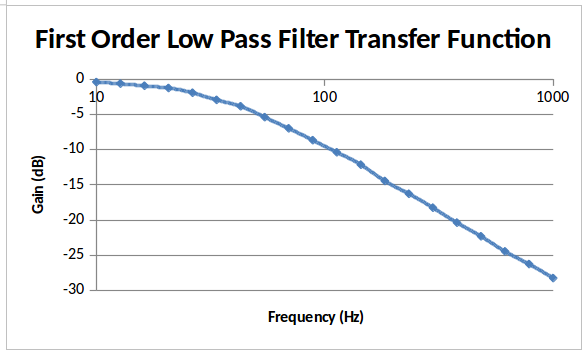
\includegraphics[width=0.5\textwidth]{FirstLow.png}
	\caption{First order low pass filter Bode Plot}
\end{figure}

\subsection*{First Order High Pass Filter}
$$f_c = 33.59Hz$$
\begin{figure}[H]
	\centering
	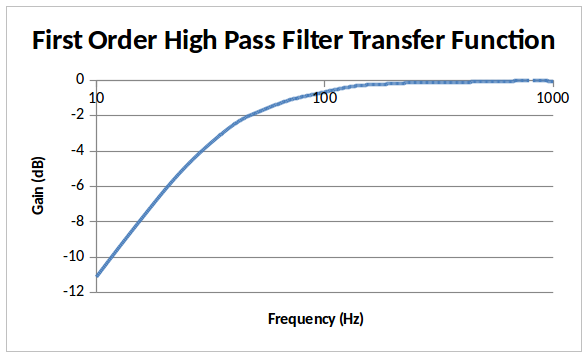
\includegraphics[width=0.5\textwidth]{FirstHigh.png}
	\caption{First order high pass filter Bode Plot}
\end{figure}

\subsection*{Second Order Low Pass Filter}
$$f_{MaxGainMeasured} = 545.6 Hz$$
\begin{figure}[H]
	\centering
	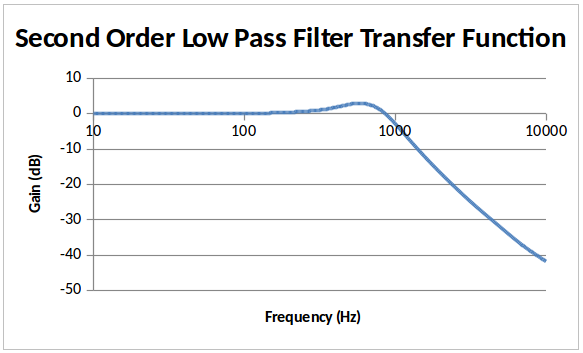
\includegraphics[width=0.5\textwidth]{SecondLow.png}
	\caption{Second order low pass filter Bode Plot}
\end{figure}

\subsection*{Second Order High Pass Filter}
$$f_{MaxGainMeasured} = 784.2 Hz$$
\begin{figure}[H]
	\centering
	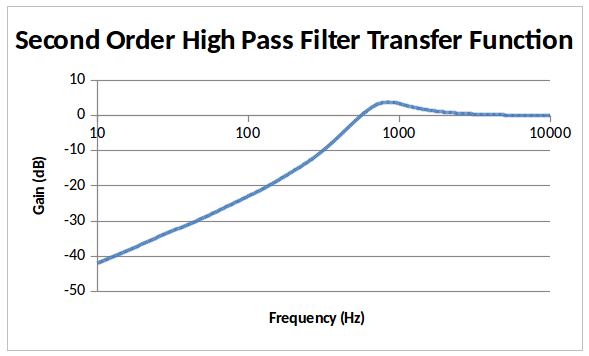
\includegraphics[width=0.5\textwidth]{SecondHigh.png}
	\caption{Second order high pass filter Bode Plot}
\end{figure}

\subsection*{Second Order Bandpass Filter}
$$f_{MaxGainMeasured} = 701.7 Hz$$
$$f_{Bandwidth} = 1012.6Hz$$
\begin{figure}[H]
	\centering
	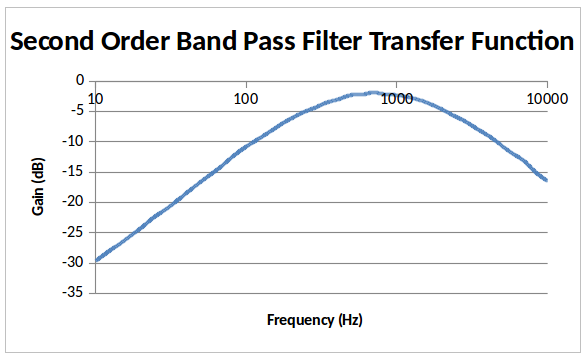
\includegraphics[width=0.5\textwidth]{SecondBandPass.png}
	\caption{Second order bandpass filter Bode Plot}
\end{figure}

\subsection*{Second Order Band Reject Filter}
$$f_{MinGainMeasured} = 701.7 Hz$$
$$f_{Bandwidth} = 1788.5Hz$$
\begin{figure}[H]
	\centering
	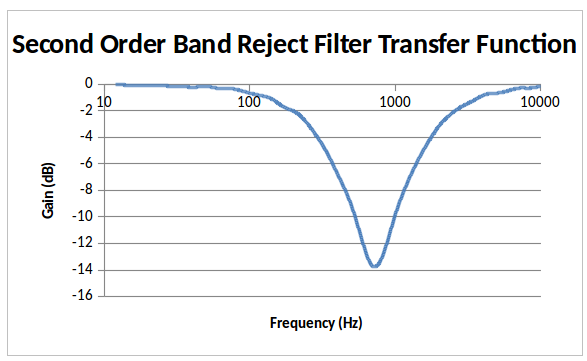
\includegraphics[width=0.5\textwidth]{SecondReject.png}
	\caption{Second order band reject filter Bode Plot}
\end{figure}

\subsection*{Second Order Band Reject Filter with Different Resistor}
$$f_{MinGainMeasured} = 701.7 Hz$$
$$f_{Bandwidth} = 9965.4Hz$$
\begin{figure}[H]
	\centering
	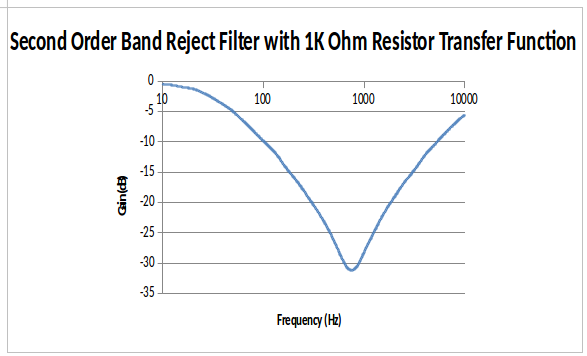
\includegraphics[width=0.5\textwidth]{SecondReject1k.png}
	\caption{Second order band reject filter with 1k $\ohm$ Bode Plot}
\end{figure}

\subsection*{Active Filters}
$$f_c = 33.59Hz$$
\begin{figure}[H]
	\centering
	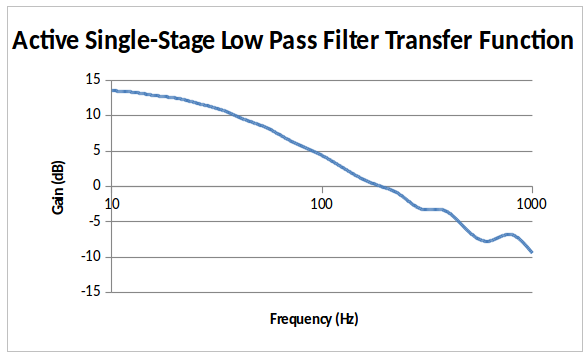
\includegraphics[width=0.5\textwidth]{SingleStage.png}
	\caption{Single stage active filter Bode Plot}
\end{figure}

\subsection*{Active Filters with More Stages}
$$f_c = 143.8Hz$$
\begin{figure}[H]
	\centering
	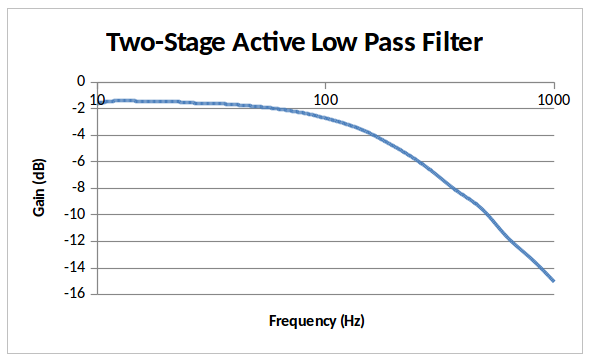
\includegraphics[width=0.5\textwidth]{TwoStage.png}
	\caption{Two stage active filter Bode Plot}
\end{figure}

\section*{Post-Lab}
\subsection*{First Order Low Pass Filter}
$Percentage Error = \frac{|measured-calculated|}{calculated} = \frac{|33.59-33.86|}{33.86} = 0.80\%$\\
\noindent The difference between our calculated and measured cutoff frequency is extremely small.

\subsection*{First Order High Pass Filter}
$Percentage Error = \frac{|measured-calculated|}{calculated} = \frac{|33.59-33.86|}{33.86} = 0.80\%$\\
\noindent The difference between our calculated and measured cutoff frequency is extremely small.

\subsection*{Second Order Low Pass Filter}
$Percentage Error = \frac{|measured-calculated|}{calculated} = \frac{|545.6-734|}{734} = 25.67\%$\\
\noindent The difference between our calculated and measured cutoff frequency is fairly high. This is most likely due to inaccurate use of the cursors in both LTSpice and the lab software.\\

\noindent The gain of the second order low pass filter decreases at a faster rate than the first order low pass filter, however, the second order low pass filter has a larger overshoot than the first order low pass filter. The first order low pass filter is better for uses where a low overshoot is needed, while the second order low pass filter is better for uses where a large rate of decrease is needed, and an overshoot is allowable.

\subsection*{Second Order High Pass Filter}
$Percentage Error = \frac{|measured-calculated|}{calculated} = \frac{|784.2-734|}{734} = 6.84\%$\\
\noindent The difference between our calculated and measured cutoff frequency is fairly low.\\

\noindent Both the theoretical and experimental Bode plots show similar slopes within the specified stop-band.\\

\noindent The gain of the second order high pass filter decreases at a faster rate than the first order high pass filter, however, the second order high pass filter has a larger overshoot than the first order high pass filter. The first order high pass filter is better for uses where a low overshoot is needed, while the second order high pass filter is better for uses where a large rate of decrease is needed, and an overshoot is allowable.\\

\noindent Increasing the resistance will result in a higher bandwidth, while decreasing the resistance will result in a lower bandwidth. It will have no effect on the frequency of maximum gain.

\subsection*{Second Order Bandpass Filter}
$Percentage Error = \frac{|measured-calculated|}{calculated} = \frac{|701.7-734|}{734} = 4.40\%$\\
$Percentage Error = \frac{|measured-calculated|}{calculated} = \frac{|1012.6-1600|}{1600} = 0.37\%$\\\
\noindent The difference between our calculated and measured maximum gain frequency is fairly low. Additionally, the difference between our calculated and measured bandwith is fairly low.

\subsection*{Second Order Band Reject Filter}
$Percentage Error = \frac{|measured-calculated|}{calculated} = \frac{|701.7-734|}{734} = 4.40\%$\\
$Percentage Error = \frac{|measured-calculated|}{calculated} = \frac{|1788.5-1591|}{1591} = 12.41\%$\\
\noindent The difference between our calculated and measured minimum gain frequency is fairly low. Additionally, the difference between our calculated and measured bandwith is fairly low.

\subsection*{Second Order Band Reject Filter with Different Resistor}
$f_{MinGain} = 734Hz$\\
$Bandwidth = 15900Hz$\\
$Percentage Error = \frac{|measured-calculated|}{calculated} = \frac{|701.7-734|}{734} = 4.40\%$\\
$Percentage Error = \frac{|measured-calculated|}{calculated} = \frac{|9965.4-15900|}{15900} = 37.32\%$\\
\noindent The difference between our calculated and measured minimum gain frequency is fairly low. Additionally, the difference between our calculated and measured bandwith is fairly high. This is most likely due to inaccurate use of the cursors in both LTSpice and the lab software.

\subsection*{Active Filters}
$f_c = 33.86 Hz$\\
$Percentage Error = \frac{|measured-calculated|}{calculated} = \frac{|33.59-33.86|}{33.86} = 0.80\%$\\
\noindent The difference between our calculated and measured cutoff frequency is extremely small.\\

\noindent The active filter has a similar rate of decrease in gain as the first order low pass filter, but has a lower rate of decrease in gain as the second order low pass filter. Additionally, it has a positive gain, while both the first and second order low pass filters begin at a gain very close to zero. The active circuit allows for positive gain, but dictates a second power supply. Additionally, it does not have any offshoot.\\

\subsection*{Active Filters with More Stages}
\noindent The two stage active filter has a similar rate of decrease in gain as the first order low pass filter, but has a lower rate of decrease in gain as the second order low pass filter. The gain begins at a negative number, and the cutoff of the filter is lower than the single stage active filter. The two stage filter has the same disadvantages as a single stage filter. However, it would excel in areas which require low frequencies and low overshoot.
\end{document}